\documentclass[notheorems,mathserif,table,compress]{beamer}  %dvipdfm选项是关键,否则编译统统通不过
%%------------------------常用宏包------------------------
%%注意, beamer 会默认使用下列宏包: amsthm, graphicx, hyperref, color, xcolor, 等等
\usepackage{fontspec,xunicode,xltxtra}  % for XeTeX
\usepackage{comment}
\usepackage{fancybox}
%%------------------------ThemeColorFont------------------------
%% Presentation Themes
% \usetheme[<options>]{<name list>}
\usetheme{Madrid}
%% Inner Themes
% \useinnertheme[<options>]{<name>}
%% Outer Themes
% \useoutertheme[<options>]{<name>}
\useoutertheme{miniframes} 
%% Color Themes 
% \usecolortheme[<options>]{<name list>}
%% Font Themes
% \usefonttheme[<options>]{<name>}
\setbeamertemplate{background canvas}[vertical shading][bottom=white,top=structure.fg!7] %%背景色, 上25%的蓝, 过渡到下白.
\setbeamertemplate{theorems}[numbered]
\setbeamertemplate{navigation symbols}{}   %% 去掉页面下方默认的导航条.
\usepackage{zhfontcfg}
%\setsansfont[Mapping=tex-text]{文泉驿正黑}  %% 需要fontspec宏包
     %如果装了Adobe Acrobat,可在font.conf中配置Adobe字体的路径以使用其中文字体
     %也可直接使用系统中的中文字体如SimSun,SimHei,微软雅黑 等
     %原来beamer用的字体是sans family;注意Mapping的大小写,不能写错
     %设置字体时也可以直接用字体名,以下三种方式等同:
     %\setromanfont[BoldFont={黑体}]{宋体}
     %\setromanfont[BoldFont={SimHei}]{SimSun}
     %\setromanfont[BoldFont={"[simhei.ttf]"}]{"[simsun.ttc]"}
%%------------------------MISC------------------------
\graphicspath{{figures/}}         %% 图片路径. 本文的图片都放在这个文件夹里了.
%%------------------------正文------------------------
\begin{document}
\XeTeXlinebreaklocale "zh"         % 表示用中文的断行
\XeTeXlinebreakskip = 0pt plus 1pt % 多一点调整的空间
%%----------------------------------------------------------
%% This is only inserted into the PDF information catalog. Can be left
%% out.
%%%
%% Delete this, if you do not want the table of contents to pop up at
%% the beginning of each subsection:
\begin{comment}
\AtBeginSection[]{                              % 在每个Section前都会加入的Frame
  \frame<handout:0>{
    \frametitle{Content}\small
    \tableofcontents[current,currentsubsection]
  }
}
\AtBeginSubsection[]                            % 在每个子段落之前
{
  \frame<handout:0>                             % handout:0 表示只在手稿中出现
  {
    \frametitle{下一节内容}\small
    \tableofcontents[current,currentsubsection] % 显示在目录中加亮的当前章节
  }
}
\end{comment}
%%----------------------------------------------------------
\title[每周汇报之新人篇]{每周汇报之新人篇}
\subtitle{---我们是菜鸟}
\author[CVBIOUC]{主讲人~~~~~\textcolor{olive}{赵海伟\ 戴嘉伦\ 王如晨}\\
    \quad 幻灯片制作~~\textcolor{olive}{赵海伟\ 戴嘉伦\ 王如晨}}
\institute[Ocean University of China]{\small\textcolor{violet}{中国海洋大学~~信息科学与工程学院}}
\date{\today}
%\titlegraphic{\vspace{-6em}\includegraphics[height=7cm]{ouc}\vspace{-6em}}
\frame{ \titlepage }
%%----------------------------------------------------------
%\section*{目录}
\frame{\frametitle{content}\tableofcontents}
%%----------------------------------------------------------

%\section{Beamer类和XeTeX概览} %如果你想书签不出现问题,请不要用\XeTeX
                                 %这类复杂的指令,直接写XeTeX吧
\section{中国海洋大学2014级研究生奖助学金政策解读}

\begin{frame}
  \frametitle{2014级研究生奖学金体系}
  \begin{figure}[!ht]
  \centering\includegraphics[width=1.8in]{m.png}
  \caption{研究生奖学金体系之国家奖学金\&学业奖学金}
  \end{figure} 
\end{frame}

\begin{frame}
  \frametitle{2014级研究生奖学金体系}
  \begin{figure}[!ht]
  \centering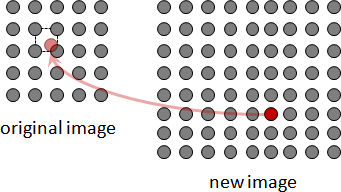
\includegraphics[width=3in]{n.png}
  \caption{研究生奖学金体系之专项奖学金}
  \end{figure} 
\end{frame}

\begin{frame}
  \frametitle{2014级研究生资助体系}
  \begin{figure}[!ht]
  \centering\includegraphics[width=2in]{o.png}
  \caption{研究生资助体系之国家助学金\&三助}
  \end{figure} 
\end{frame}

\begin{frame}
  \frametitle{2014级研究生资助体系}
  \begin{figure}[!ht]
  \centering\includegraphics[width=2in]{p.png}
  \caption{研究生资助体系之国家助学贷款\&经济困难研究生补助}
  \end{figure} 
\end{frame}

\section{Linux操作系统安装及使用}

\subsection{Linux操作系统安装之前配置}

\begin{frame}
  \frametitle{Linux操作系统安装之前配置}
   vim /proc/cpuinfo
  \begin{figure}[!ht]
  \centering\includegraphics[width=3.5in]{cpu.png}
  \caption{查看CPU性能}
  \end{figure} 
\end{frame}

\subsection{Linux操作系统的安装}

\begin{frame}
  \frametitle{Linux操作系统的安装}
  \begin{figure}[!ht]
  \centering\includegraphics[width=3.5in]{a.png}
  \caption{语言选择}
  \label{fig:1}
  \end{figure}
\end{frame}
  
\begin{frame}
  \frametitle{Linux操作系统的安装}
  \begin{figure}[!ht]
  \centering\includegraphics[width=3.5in]{b.png}
  \caption{检查准备情况}
  \label{fig:2}
  \end{figure}
\end{frame}

\begin{frame}
  \frametitle{Linux操作系统的安装}  
  \begin{figure}[!ht]
  \centering\includegraphics[width=3.5in]{c.png}
  \caption{磁盘分区}
  \label{fig:3}
  \end{figure}
\end{frame}

\begin{frame}
  \frametitle{Linux操作系统的安装}  
  \begin{figure}[!ht]
  \centering\includegraphics[width=3.5in]{d.png}
  \caption{磁盘分区}
  \label{fig:4}
  \end{figure}
\end{frame}

\begin{comment}
  \frametitle{Linux操作系统的安装}  
  \begin{itemize}
  \item 交换分区:4G
  \item / :50G\\
        存放安装的系统
  \item /opt:50G\\
        存放安装的软件
  \item /home:剩余空间\\
        存放数据文件
  \end{itemize}
\end{comment}

\begin{frame}

\begin{table}[!htp] %插表
\label{tab:1}
\centering
\begin{tabular}{|c|c|c|}
\hline
交换分区&4G&虚拟内存\\
\hline
/ &50G&存放安装的系统\\
\hline
/opt&50G&存放安装的软件\\
\hline
/home&剩余空间&存放数据文件\\
\hline
\end{tabular}  
\caption{Linux操作系统安装中的磁盘分区}
\end{table}

\end{frame}

\begin{frame}
  \frametitle{Linux操作系统的安装}  
  \begin{figure}[!ht]
  \centering\includegraphics[width=3.5in]{e.png}
  \label{fig:5}
  \caption{开始安装}
  \end{figure}
\end{frame}

\begin{frame}
  \frametitle{Linux操作系统的安装}  
  \begin{figure}[!ht]
  \centering\includegraphics[width=3.5in]{f.png}
  \label{fig:6}
  \caption{设置键盘布局}
  \end{figure}
\end{frame}

\begin{frame}
  \frametitle{Linux操作系统的安装}  
  \begin{figure}[!ht]
  \centering\includegraphics[width=3.5in]{g.png}
  \caption{设定用户名密码} 
  \label{fig:7}
  \end{figure}
\end{frame}

\begin{frame}
  \frametitle{Linux操作系统的安装}  
  \begin{figure}[!ht]
  \centering\includegraphics[width=3.5in]{h.png}
  \caption{网络设置}
  \label{fig:8}
  \end{figure}
\end{frame}

\begin{frame}
  \frametitle{Linux操作系统的安装}  
  \begin{figure}[!ht]
  \centering\includegraphics[width=3.5in]{i.png}
  \caption{网络设置}
  \label{fig:9}
  \end{figure}
\end{frame}

\begin{frame}
  \frametitle{Linux操作系统的安装}  
  \begin{figure}[!ht]
  \centering\includegraphics[width=3.5in]{j.png}
  \caption{网络设置}
  \label{fig:10}
  \end{figure} 
\end{frame}

\begin{frame}
  \frametitle{Linux操作系统的安装}  
  \begin{itemize}
  \item IP:222.195.148.88(每个人的IP最后一位不同)
  \item 网关:222.195.149.254
  \item 子网掩码:255.255.254.0
  \item DNS服务器:211.64.142.6
  \end{itemize}
\end{frame}

\subsection{Linux操作系统下软件的安装}

\begin{frame}
  \frametitle{Linux操作系统下利用索引进行软件的下载及安装}
  \begin{itemize}
  \item 索引更新:sudo apt-get update
  \item 通过索引下载软件:sudo apt-get install iptux(信使)
  \end{itemize}
\end{frame}

\begin{frame}
  \frametitle{信使的安装及使用}  
  \begin{figure}[!ht]
  \centering\includegraphics[width=3.5in]{k.png}
  \caption{利用信使传送文件}
  \label{fig:11}
  \end{figure}
\end{frame}

\begin{frame}
  \frametitle{信使的安装及使用}  
  \begin{figure}[!ht]
  \centering\includegraphics[width=3.5in]{l.png}
  \caption{利用信使传送文件}
  \label{fig:12}
  \end{figure}
\end{frame}

\begin{frame} 
  \frametitle{Linux操作系统下设置开机挂载进行软件的安装}
  \begin{itemize}
  \item 挂载:sudo mount -o loop /路径/x.iso /mnt
  \item 取消挂载:unmount /路径/x.iso(或者/mnt)
  \end{itemize}
\end{frame}

\subsection{vim编辑器的安装及使用}

\begin{frame}
  \frametitle{vim编辑器的安装及使用}
  \begin{itemize}
  \item 索引更新:sudo apt-get update
  \item 利用索引下载软件:sudo apt-get install vim(软件名)
  \end{itemize}
\end{frame}


\begin{frame}
  \frametitle{vim编辑器的安装及使用}
  \begin{itemize}
  \item 创建文件:touch text.txt
  \item 打开文件:vim text.txt
  \item 按i键进行文本编辑
  \item 按ESC键退出编辑模式
  \item 保存::w 保存后退出::x 强制保存::w! 强制退出不保存::q! 退出::q
  \end{itemize}
\end{frame}

\subsection{Linux操作系统下的部分指令}

\begin{frame} 
  \frametitle{Linux文件权限概念}
  \begin{itemize}
  \item sudo 指令
  \item sudo chmod 777 指令
  \end{itemize}
\end{frame}

\begin{frame} 
  \frametitle{目录与路径}
  \begin{itemize}
  \item 当前用户的主目录:$\sim$=/home/zhaohaiwei
  \item 根目录:/
  \item 补全:Tab
  \item 转换目录:cd /home/zhaohaiwei/software
  \item 进入上一层目录:cd ..
  \item 重新命名文件夹:mv a b
  \end{itemize}
\end{frame}

\begin{frame} 
  \frametitle{文件与目录管理}
  \begin{itemize}
  \item 新建文件夹:mkdir 文件夹名称
  \item 移动文件夹:mv /A /B(将A文件夹移动到B路径下)
  \item 移动当前路径下全部到B路径下: mv * /B
  \item 删除文件夹:rm /B
  \item 删除文件夹内包含子目录的全部:rm -rf /B
  \item 删除当前路径下全部:rm -r 文件名
  \item 删除当前路径下名称包含.so的文件:rm -r(递归) *.so*
  \item 复制文件夹:cp -r /A /B
  \end{itemize}
\end{frame}

\begin{frame} 
  \frametitle{文件内容查阅}
  \begin{itemize}
  \item 查看当前目录内容:ls
  \item 查看当前目录所有内容(包含隐藏文件):ls -a
  \end{itemize}
\end{frame}

\section{Linux操作系统下Matlab的安装}

\begin{frame}
  \frametitle{Matlab安装步骤}
  sudo mount -o loop Matlab.iso /mnt   
    \begin{itemize}
    \item  mount 为挂上,挂载    mnt为mount的缩写
    \item  -o option <选项>    -t  type   <文件类型>
    \item  loop是mount用来加载loop设备的选项,用来把一个文件当成硬盘分区挂接上系统 
    \item  umount为退出挂载指令  /mnt
    \end{itemize}
\end{frame}



\begin{frame}
  \frametitle{安装步骤}
  \begin{enumerate}
  \item cd /mnt  进入挂载目录 
  \item sudo ./install    
  \item 在安装过程中,修改安装路径
  \item 执行sudo /opt/matlab/bin/matlab激活程序
  \end{enumerate}
\end{frame}



\begin{frame}
 \frametitle{Matlab创建快捷方式}
  创建并编辑Matlab.desktop  输入以下内容 \\
  sudo gedit /usr/share/applications/Matlab.desktop\\
  \lbrack Desktop Entry\rbrack\\
  Type=Application\\
  Name=Matlab\\
  GenericName=Matlab 2013a\\
  Comment=Matlab:The Language of Technical Computing\\
  Exec=sh /opt/matlab/bin/matlab -desktop\\
  Icon=/opt/matlab/toolbox/nnet/nnresource/icons/matlab.png\\
  Terminal=false\\
  Categories=Development;Matlab;
\end{frame}

\begin{frame}
 \frametitle{Matlab解决中文乱码问题}
  \begin{enumerate}
  \item 确定自己的jre目录路径 /opt/matlab/sys/java/jre/glnx86/jre 
  \item 进入字体库 cd /opt/matlab/sys/java/jre/glnx86/jre/lib/fonts
  \item 建立字体目录fallback: mkdir fallback
  \item 把字体复制到fallback目录: cp /usr/share/fonts/truetype/wqy ./fallback
  \item 在fallback下,执行 mkfontscale 命令,生成fonts.scale;
  \item 添加文件  cat fallback/fonts.scale >> fonts.dir 
  \item 把fallback下的字体加上可读属性:chmod a+r fallback/*
  \end{enumerate}
\end{frame}

\section{Linux操作系统下\LaTeX{}的安装使用}
\begin{frame}
  \frametitle{\LaTeX{}}
 \hspace{2em}  \LaTeX{}是一种基于TeX的排版系统,利用这种格式,即使使用者没有排版和程序设计的知识也可以充分发挥由TeX所提供的强大功能,能在几天,甚至几小时内生成很多具有书籍质量的印刷品。对于生成复杂表格和数学公式,这一点表现得尤为突出。因此它非常适用于生成高印刷质量的科技和数学类文档。这个系统同样适用于生成从简单的信件到完整书籍的所有其他种类的文档。
\end{frame}


\begin{frame}
  \frametitle{\LaTeX{}安装步骤}
  \begin{enumerate}
  \item 挂载镜像文件:\\
  sudo mount -o loop ~/software/texlive2013.iso /mnt
  \item 在终端输入:
      \begin{itemize}
      \item   cd /mnt
      \item   sudo ./install-tl
      \end{itemize}
  \item 安装后默认的安装目录是/usr/local,要把安装文件移动到/opt下:
  mv /usr/local/texlive /opt
  \end{enumerate}
\end{frame}

\begin{frame}
  \frametitle{\LaTeX{}修改配置}
  \begin{enumerate}
  \item 打开终端,输入:sudo vim ~/.profile 或者/.bashrc
    \begin{itemize}        
    \item PATH=/opt/texlive/2013/bin/x86\_64-linux: \$PATH;export PATH
    \item MANPATH=/opt/texlive/2013/texmf-dist/doc/man: \$MANPATH;export MANPATH
    \item INFOPATH=/opt/texlive/2013/texmf-dist/doc/info: \$INFOPATH;export INFOPATH
    \end{itemize}
  \end{enumerate}
\end{frame}

\begin{frame}
  \frametitle{\LaTeX{}路径配置差异}
    \begin{itemize}        
    \item 首先读入的是全局环境变量设定档/etc/profile
    \item 根据不同使用者,首先读取 $\sim$/.bash\_profile,否则就读取$\sim$/.bash\_login,最后读取 $\sim$/.profile,这三个文档设定基本一样的,读取有优先关系
    \item $\sim$/.profile可以设定本用户专有的路径,环境变量等,它只能登入的时候执行一次
    \item $\sim$/.bashrc也是某用户专有设定文档,可以设定路径,命令别名,每次shell script的执行都会使用它一次
    \end{itemize}
\end{frame}

\begin{frame}
  \frametitle{\LaTeX{}基本语句}
  \begin{itemize}
  \item 通过宏包内指令来解决特定问题\\
     \hspace{0.5in}   $\backslash$usepackage\{option\} \{package\}
  \item 特殊字符\\
    \hspace{0.5in}\# \$ \% \_ \{\}   需要添加 $\backslash$符号
  \item 注释多行 \\
    \hspace{0.5in}   $\backslash$begin\{comment\}  \\
    \hspace{0.5in}   $\backslash$end\{comment\}
  \item  空白距离\\
    \hspace{0.5in}   $\backslash$hspace\{尺寸\} 
  \end{itemize}
\end{frame}

\begin{frame}
  \frametitle{基本语句}
  \begin{itemize}
  \item itemize适用简单列表   enumerate适用有序列表   \\
        description适用带描述列表
  \item  插入图片
    \begin{itemize}
    \item $\backslash$begin\{option\} figure单图 minipage并列
    \item $\backslash$includegraphics[尺寸]\{图片名字\}
    \item $\backslash$caption\{注释内容\}
    \item $\backslash$end\{option\}同上
    \end{itemize}
  \item begin与end一一对应,良好的编写结构与习惯能够减少错误
  \end{itemize}
\end{frame}

\begin{frame} 
\frametitle{修改心得}
  \begin{enumerate}
  \item 随意使用sudo后,许多普通权限的文件被提升权限,导致其他程序调用或者执行的时候出现问题,不能顺利安装程序
  \item 输入代码的时候务必细心注意,常常一个字母的输入错误,就有可能导致整个安装过程遇到困难
  \item 在命令行中进行操作时,应该注意目标文件夹或者该文件夹下的文件是否确实存在,否则出现错误往往不知道哪里出现错误
  \item 在进行软件中文字体安装的过程中,需确认系统中存在该字体库,并且软件能够显示该字体
  \item 在LaTex中许多符号是无法正常显示的,可能导致PDF文件无法正常生成,所以出现错误时务必注意特殊符号的使用
  \end{enumerate}
\end {frame}

\section{Linux操作系统下codeblocks的安装}

\begin{frame}
  \frametitle{Code::Blocks}
  是一个开放源码的C/C++集成开发环境。\\
  安装:sudo apt-get install CodeBlocks
\end{frame}

\section{Linux操作系统下OpenCV的安装}

\begin{frame}
\frametitle{OpenCV}
是一个基于开源的计算机视觉库。\\
\begin{itemize}
\item 安装\\
	\begin{enumerate}
	\item 解压——将下载的源代码包解压:unzip opencv.zip\\
	\item 进入源码目录cd opencv-2.4.9,创建release目录mkdir release\\
	\item 进入release,cmake编译Opencv,将部分编译后的文件放到/opt/opencv目录下:\\
cmake -D CMAKE\_BUILD\_TYPE=RELEASE -D CMAKE\_INSTALL\_PREFIX=/opt/opencv ..  \\
	\item sudo make install安装\\
	\end{enumerate}
\item 测试
\end{itemize}
\end{frame}

\section{GitHub的安装及使用}

\begin{frame}
\frametitle{Github}
是Git的项目托管网站,用于存放使用Git版本控制的软件代码和内容项目。\\
SSH代理:在完成从本地仓库上传材料Github或者从Github下载资料的过程中,需要利用SSH协议来防止信息的泄漏。\\
\end{frame}


\begin{frame}
\frametitle{设置SSH密钥}
\begin{itemize}
\item 执行ssh-keygen -t rsa,可以生成一个私钥文件id\_rsa.pub。
\item 将产生的文件保存在Github网站上。
	\begin{figure}
	\centering
	\includegraphics[width=3.5in]{sshkeys.png}
	\caption{SSH Keys}
	\end{figure} 
\item ssh-add把密钥加载到SSH。
\end{itemize}
\end{frame}


\begin{frame}
\frametitle{Git的安装配置}
\begin{itemize}
\item Git的安装:sudo apt-get install git
\item 配置:git config配置环境变量,可以控制Git的外观和操作等。初次运行Git要用git config --global设置用户名和邮件地址。
\end{itemize}

\end{frame}


%\section{收获感悟}
\begin{frame}
  \frametitle{Git和Github的使用}
\begin{itemize}
\item 初始化仓库:git init
\item 跟踪文件与取消跟踪:
	\begin{itemize}
	\item 跟踪文件:git add filename
	\item 取消跟踪:git rm --cached filename
	\item 查看状态:git status
	\end{itemize}
\item 提交文件:git commit -m 'message'
\end{itemize}
\end{frame}

\begin{frame}
  \frametitle{新建库并上传}
\begin{itemize}
\item 在Github网站Respositories选项卡下新建一个库Test。
\item 让Git记住远程库的名和地址:git remote add origin http://github.com/wangruchen/Test.git
\item 推送到远程库:git push origin master
\end{itemize}   
\end{frame}

\begin{frame}
  \frametitle{本地仓库与远程仓库冲突}
有时用git commit提交文件之后,再用git push提交到远程时,会出现无法推送的问题。\\
\begin{itemize}
\item 原因:远程仓库和本地版本对应不上。
\item 用git pull,就可以把Github上的新内容合并到本地,使本地仓库和远程仓库同步。然后就可以通过git push推送到远程库。
\end{itemize}       
\end{frame}

\begin{frame}
\frametitle{恢复历史版本}
Git可以记录进行操作和修改的所有版本。当有需要时,可以恢复到之前某个版本时。\\
\begin{enumerate}
\item 用git log查看想要恢复的版本的哈希值。\\
\item 用git reset加选中版本的哈希值,恢复到选中版本。\\
\end{enumerate} 
\end{frame}

\begin{frame}
\frametitle{克隆已有的仓库}
\begin{itemize}
\item 克隆:进入要建立仓库的目录,执行git clone git@github.com:zhenglab/ROC\_PR.git。
\item 提交文件
\end{itemize} 
\end{frame} 

\section{公共网盘的使用}

\begin{frame}
\frametitle{公共盘}
222.195.149.61,上面存放这各种实验室数据,以及历年博士和硕士资料。\\
服务器一共四个虚拟磁盘:data、software、research、study。\\
\begin{itemize}
\item data主要存放数据
\item software主要存放软件
\item research主要存放项目和学习资料
\item study主要存放历年毕业的博硕士资料及各种视频资料
\end{itemize}
\end{frame}

\end{document}

